\appendix

\subsection{Model Overview (Continued)}
	\begin{figure}
		\centering
		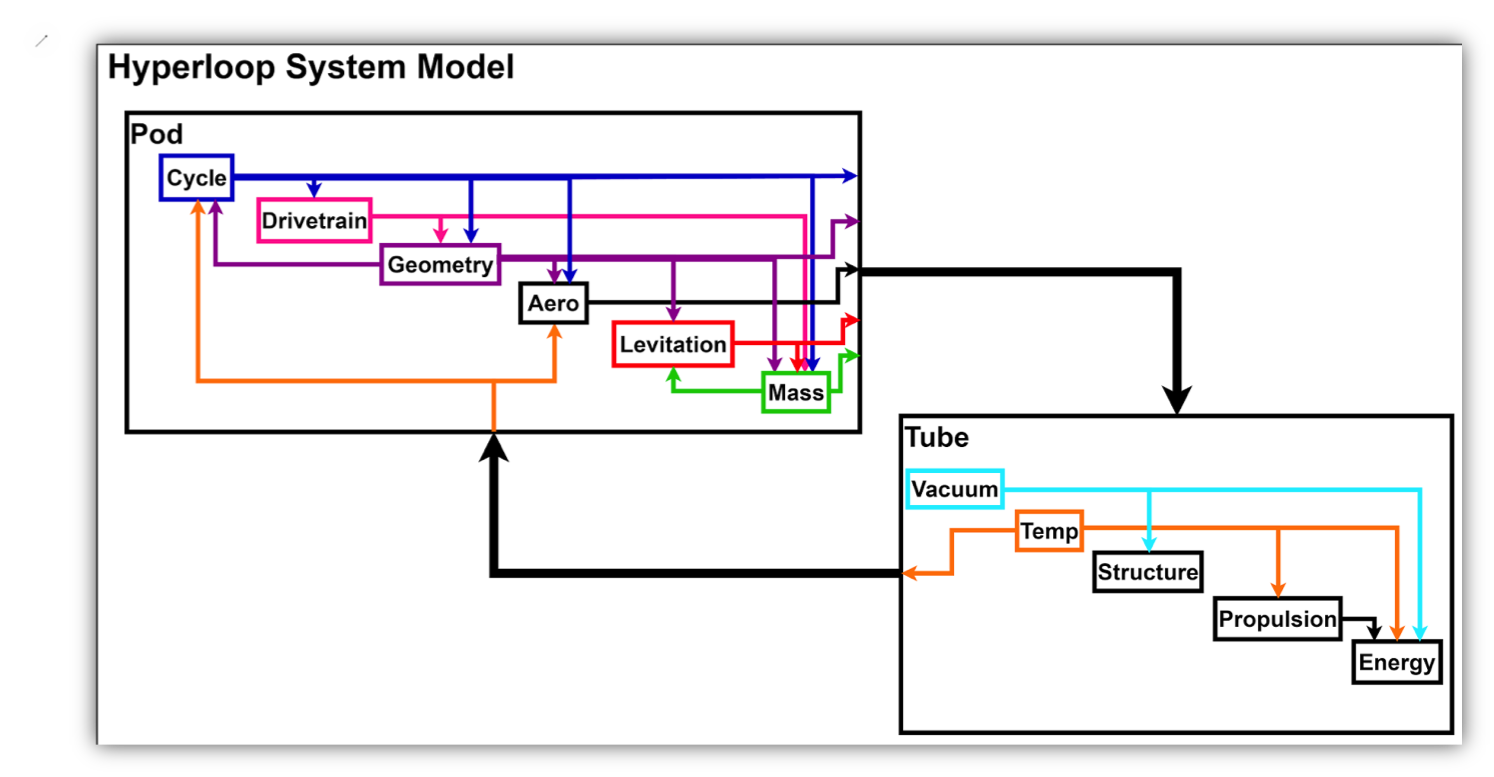
\includegraphics{../images/modelOverview.png}
		\caption{XDSM diagram for entire system model}
		\label{fig:xdsm:toplevel}
	\end{figure}}

\section{TubeGroup}
	% \begin{figure}
	% 	\centering
	% 	\includegraphics{../images/tube.png}
	% 	\caption{Hierarchial tree digram showing structure of TubeGroup}
	% 	\label{fig:tree:tube}
	% \end{figure}
	% \begin{figure}
	% 	\centering
	% 	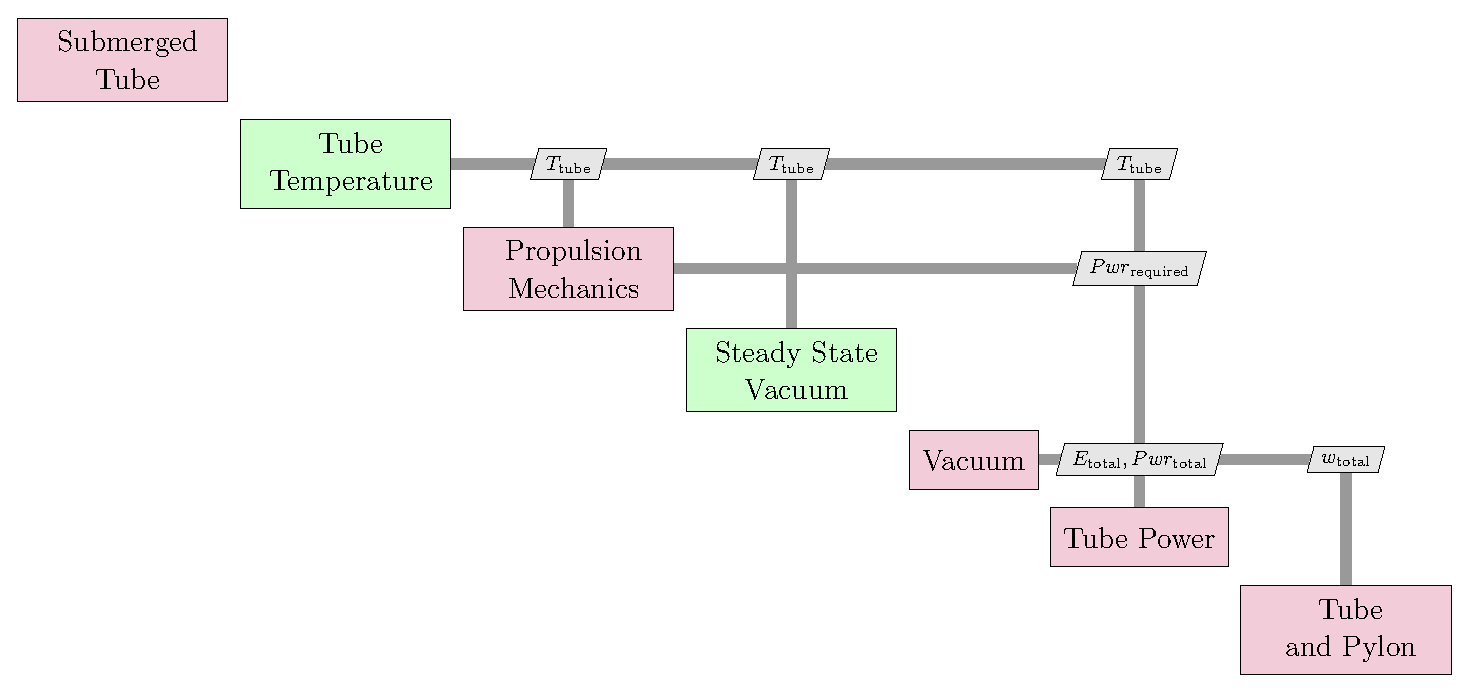
\includegraphics{../images/xdsm/tube.pdf}
	% 	\caption{XDSM diagram for Tube group}
	% 	\label{fig:xdsm:drivetrain}
	% \end{figure}}
	\subsection{PropulsionMechanics}
	\subsection{TubeTemp}
		\begin{figure}
			\centering
			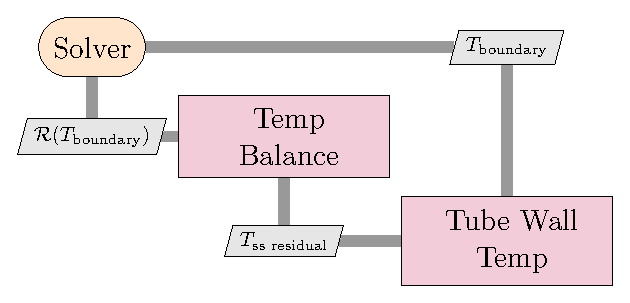
\includegraphics{../images/xdsm/temp.pdf}
			\caption{XDSM diagram for TubeTemp group}
			\label{fig:xdsm:tubetemp}
		\end{figure}}
		\subsubsection{TubeWallTemp}
			\subimport{model_overview/}{tempEqs}
		\subsubsection{TempBalance}
	\subsection{Vacuum}
		\subsubsection{SteadyStateVacuum}
			\begin{figure}
				\centering
				\includegraphics{../images/xdsm/steady_state_vacuum.pdf}
				\caption{XDSM diagram for SteadyStateVacuum group}
				\label{fig:xdsm:steadystatevacuum}
			\end{figure}}
			\subsubsubsection{FlowStart}
			\subsubsubsection{Compressor}
		\subsubsection{PumpDown}
	\subsection{TubePower}
		\subimport{model_overview/}{tube_power}
	\subsection{Structure}
		\subsubsection{SubmergedTube}
		\subsubsection{TubeAndPylon}
\section{PodGroup}
	% \begin{figure}
	% 	\centering
	% 	\includegraphics{../images/pod.png}
	% 	\caption{Hierarchial tree digram showing structure of PodGroup}
	% 	\label{fig:tube}
	% \end{figure}
	% \begin{figure}
	% 	\centering
	% 	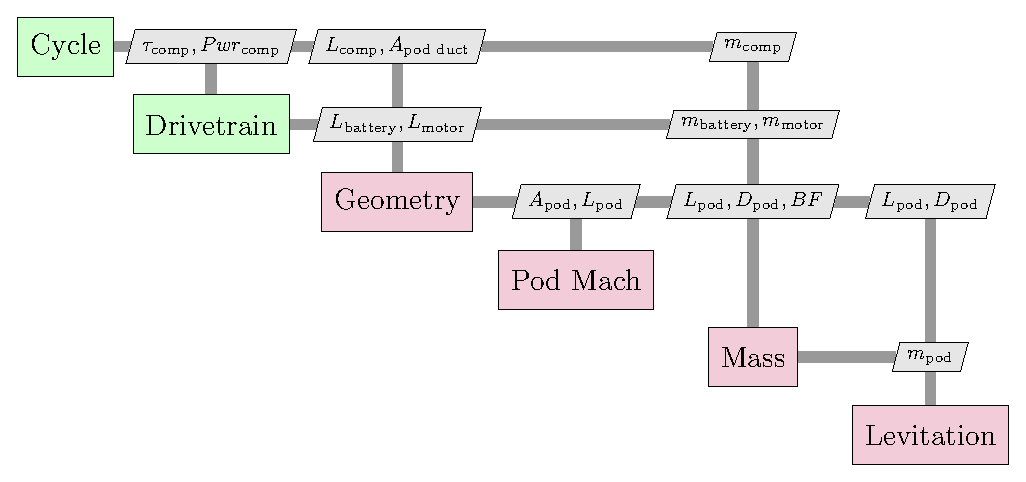
\includegraphics{../images/xdsm/pod.pdf}
	% 	\caption{XDSM diagram for Pod group}
	% 	\label{fig:xdsm:pod}
	% \end{figure}}
	\subsection{Drivetrain}
		\begin{figure}
			\centering
			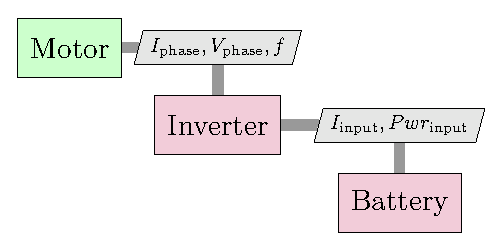
\includegraphics{../images/xdsm/drivetrain.pdf}
			\caption{XDSM diagram for Drivetrain group}
			\label{fig:xdsm:drivetrain}
		\end{figure}
		\subsubsection{Motor}
			\begin{figure}
				\centering
				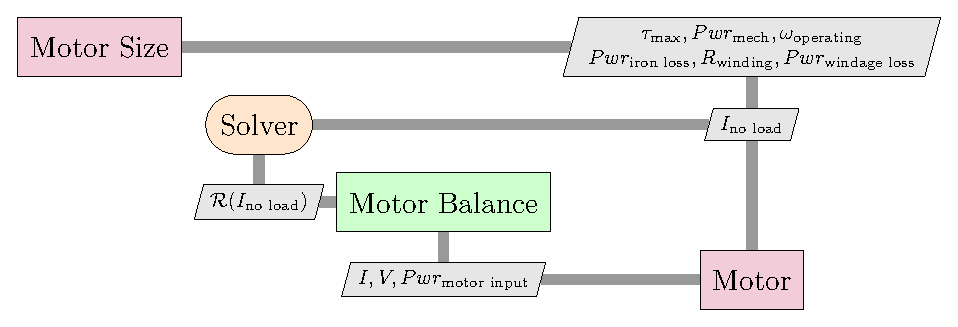
\includegraphics{../images/xdsm/motor.pdf}
				\caption{XDSM diagram for Motor group}
				\label{fig:xdsm:motor}
			\end{figure}}
			\subsubsubsection{MotorSize}
			\subsubsubsection{MotorBalance}
			\subsubsubsection{Motor}
		\subsubsection{Inverter}
		\subsubsection{Battery}
	\subsection{PodGeometry}
	\subsection{Cycle}
		\begin{figure}
			\centering
			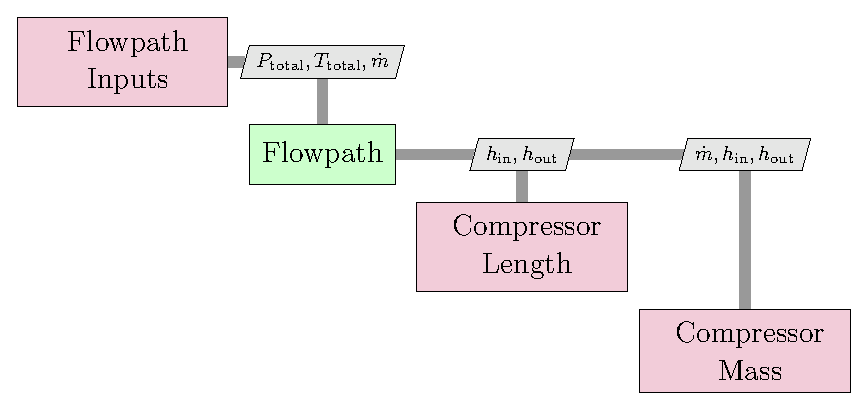
\includegraphics{../images/xdsm/cycle.pdf}
			\caption{XDSM diagram for Cycle group}
			\label{fig:xdsm:cycle}
		\end{figure}
		\subsubsection{Flowpath}
			\begin{figure}
				\centering
				\includegraphics{../images/xdsm/flowpath.pdf}
				\caption{XDSM diagram for Flowpath group}
				\label{fig:xdsm:flowpath}
			\end{figure}}
			\subsubsubsection{CompressorLength}
			\subsubsubsection{CompressorMass}
			\subsubsubsection{FlowpathInputs}
			\ssubsection{LevGroup}
			\begin{figure}
				\centering
				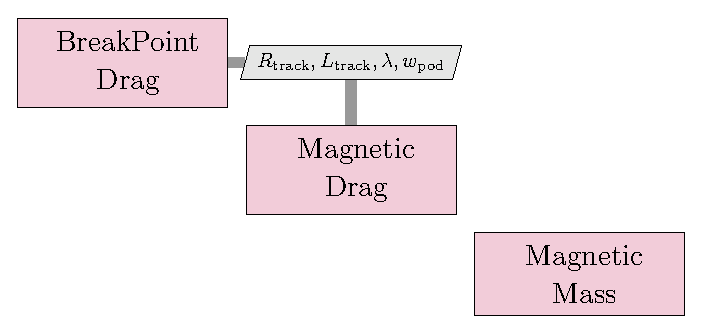
\includegraphics{../images/xdsm/levitation.pdf}
				\caption{XDSM diagram for the LevGroup group}
				\label{fig:xdsm:levitation}
			\end{figure}}
		\subsubsection{BreakpointDrag}
		\subsubsection{MagneticDrag}
		\subsubsection{MagneticMass}
	\subsection{Drag}
	\subsection{PodMach}
	\subsection{PodMass}
\section{TicketCost}
\section{SampleMission}

%from model_overview.tex
% Define all the styles used to produce XDSMs for MDO

\tikzstyle{every node}=[font=\rmfamily]

% Component types
\tikzstyle{Optimization} = [rounded rectangle,draw,fill=blue!20,inner sep=6pt,minimum height=1cm,text badly centered]
\tikzstyle{LP_Optimization} = [rectangle,draw,fill=blue!20,inner sep=6pt,minimum height=1cm,text badly centered]
\tikzstyle{Analysis} = [rectangle,draw,fill=green!20,inner sep=6pt,minimum height=1cm,text badly centered]
\tikzstyle{AnalysisGroup} = [rounded rectangle,draw,fill=green!20,inner sep=6pt,minimum height=1cm,text badly centered]
\tikzstyle{ImplicitAnalysis} = [rectangle,draw,fill=red!20,inner sep=6pt,minimum height=1cm,text badly centered]
\tikzstyle{Function} = [rectangle,draw,fill=purple!20,inner sep=6pt,minimum height=1cm,text badly centered]
\tikzstyle{FunctionGroup} = [rounded rectangle,draw,fill=red!20,inner sep=6pt,minimum height=1cm,text badly centered]
\tikzstyle{MDA} = [rounded rectangle,draw,fill=orange!20,inner sep=6pt,minimum height=1cm,text badly centered]
\tikzstyle{Metamodel} = [rectangle,draw,fill=yellow!20,inner sep=6pt,minimum height=1cm,text badly centered]
\tikzstyle{DOE} = [rounded rectangle,draw,fill=yellow!20,inner sep=6pt,minimum height=1cm,text badly centered]
%\tikzstyle{OptFunction} = [rectangle,draw,fill=red!20,inner sep=6pt,minimum height=1cm,text badly centered]

%% A simple command to give the repeated structure look for components and data
\tikzstyle{stack} = [double copy shadow]

%% A simple command to fade components and data, e.g. demonstrating a sequence of steps in an animation
\tikzstyle{faded} = [draw=black!50,fill=white,text opacity=0.5]

%% Simple fading commands for the lines
\tikzstyle{fadeddata} = [color=black!20]
\tikzstyle{fadedprocess} = [color=black!50]

% **OLD** Component types for repeated structures (i.e. for parallel structures)
%\tikzstyle{Optimization_i} = [double copy shadow, Optimization]
%\tikzstyle{LP_Optimization_i} = [double copy shadow, LP_Optimization]
%\tikzstyle{Analysis_i} = [double copy shadow, Analysis]
%\tikzstyle{Function_i} = [double copy shadow, Function]
%\tikzstyle{MDA_i} = [double copy shadow, MDA]
%\tikzstyle{Metamodel_i} = [double copy shadow, Metamodel]
%\tikzstyle{DOE_i} = [double copy shadow, DOE]

% **OLD** Faded component types for, e.g. demonstrations of each step. We use these style definitions to "gray out" large parts of the diagram.
%\tikzstyle{Optimization_fade} = [Optimization,fill=blue!10,draw=black!30,text opacity=0.3]
%\tikzstyle{Analysis_fade} = [Analysis,fill=green!10,draw=black!30,text opacity=0.3]
%\tikzstyle{Function_fade} = [Function,fill=purple!10,draw=black!30,text opacity=0.3]
%\tikzstyle{MDA_fade} = [MDA,fill=orange!10,draw=black!30,text opacity=0.3]
%\tikzstyle{Metamodel_fade} = [Metamodel,fill=yellow!10,draw=black!30,text opacity=0.3]
%\tikzstyle{DOE_fade} = [DOE,fill=yellow!10,draw=black!30,text opacity=0.3]
%
%\tikzstyle{Optimization_i_fade} = [Optimization_i,fill=blue!10,draw=black!30,text opacity=0.3]
%\tikzstyle{Analysis_i_fade} = [Analysis_i,fill=green!10,draw=black!30,text opacity=0.3]
%\tikzstyle{Function_i_fade} = [Function_i,fill=purple!10,draw=black!30,text opacity=0.3]
%\tikzstyle{MDA_i_fade} = [MDA_i,fill=orange!10,draw=black!30,text opacity=0.3]
%\tikzstyle{Metamodel_i_fade} = [Metamodel_i,fill=yellow!10,draw=black!30,text opacity=0.3]
%\tikzstyle{DOE_i_fade} = [DOE_i,fill=yellow!10,draw=black!30,text opacity=0.3]

% Data types
\tikzstyle{DataInter} = [trapezium,trapezium left angle=75,trapezium right angle=105,draw,fill=black!10]
\tikzstyle{DataIO} = [trapezium,trapezium left angle=75,trapezium right angle=105,draw,fill=white]

% **OLD** Data types for repeated structures
%\tikzstyle{DataInter_i} = [double copy shadow, DataInter]
%\tikzstyle{DataIO_i} = [double copy shadow, DataIO]

% **OLD** Faded data types
%\tikzstyle{DataInter_fade} = [DataInter,draw=black!30,fill=white,text opacity=0.3]
%\tikzstyle{DataIO_fade} = [DataIO_i,draw=black!30,fill=white,text opacity=0.3]
%
%\tikzstyle{DataInter_i_fade} = [DataInter_i,draw=black!30,fill=white,text opacity=0.3]
%\tikzstyle{DataIO_i_fade} = [DataIO_i,draw=black!30,fill=white,text opacity=0.3]

% Edges
\tikzstyle{DataLine} = [color=black!40,line width=5pt]
\tikzstyle{ProcessHV} = [-,line width=1pt,to path={-| (\tikztotarget)}]
\tikzstyle{ProcessTip} = [-,line width=1pt]

% **OLD** Faded edges
%\tikzstyle{DataLine_fade} = [DataLine,color=black!10]
%\tikzstyle{ProcessHV_fade} = [ProcessHV,color=black!30]
%\tikzstyle{ProcessTip_fade} = [ProcessTip,color=black!30]

% Matrix options
\tikzstyle{MatrixSetup} = [row sep=3mm, column sep=2mm]

% Declare a background layer for showing node connections
\pgfdeclarelayer{data}
\pgfdeclarelayer{process}
\pgfsetlayers{data,process,main}

% A new command to split the component text over multiple lines
\newcommand{\TwolineComponent}[3]
{
    \begin{minipage}{#1}
    \begin{center}
        #2 \linebreak #3
    \end{center}
    \end{minipage}
}

\newcommand{\ThreelineComponent}[4]
{
    \begin{minipage}{#1}
    \begin{center}
        #2 \linebreak #3 \linebreak #4
    \end{center}
    \end{minipage}
}

% A new command to split the component text over multiple columns
\newcommand{\MultiColumnComponent}[5]
{
    \begin{minipage}{#1}
    \begin{center}
    #2 \linebreak #3
    \end{center}
    \begin{minipage}{0.49\textwidth}
    \begin{center}
    #4
    \end{center}
    \end{minipage}
    \begin{minipage}{0.49\textwidth}
    \begin{center}
    #5
    \end{center}
    \end{minipage}
    \end{minipage}
}

\usetikzlibrary{arrows,chains,positioning,scopes,shapes.geometric,shapes.misc,shadows}
\begin{figure}
	\centering
	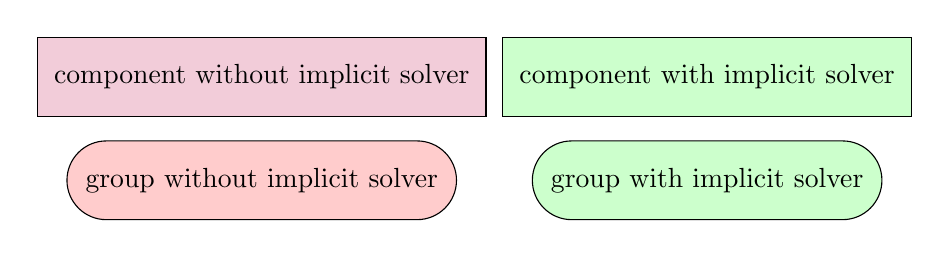
\begin{tikzpicture}
		\matrix[MatrixSetup]
		{
			\node [Function] (ExplicitComponent) {component without implicit solver}; &  \node [Analysis] (ImplicitComponent) {component with implicit solver}; \\
			\node [FunctionGroup] (ExplicitComponent) {group without implicit solver}; & \node [AnalysisGroup] (ImplicitGroup) {group with implicit solver}; \\
		};
	\end{tikzpicture}
	\label{fig:key}
\end{figure}

% from flight_frequency.tex
\begin{equation}
	\label{eq:linear_acceleration}
	Insert Linear Acceleration Equations
\end{equation}
\end{equation}
Assuming a braking deceleration of 1g, a Mach number of .8, and a tunnel
temperature of 320 K \cite{Chin}, the minimum distance between pods is
calculated to be 4.2 km with no safety margin. At top speed, the deceleration
time is calculated to be 29.2 s.


